\subsection{Система за активно следене, която използва IEEE 802.15.4 базирани ултразвукови сензори}

В документ \cite{yonei} е имплементирана система за следене на обект в пространството използвайки IEEE 802.15.4 базирани ултразвукови сензори.
IEEE 802.15.4 се използва главно в безжичните сензорни мрежи заради ниската консумация на енергия и бързия обмен на информация между компонентите на системата [фиг. \ref{fig:yoneiFig}]. Системата съдържа 1 движещ се компонент. Координатите на движещия се компонент се изчисляват чрез използване на трилатерация.  Описани са 2 категории системи за обработка и изпращане на ултразвукови сигнали \cite{sysTypes}:

\begin{enumerate}
    \item Активни - движещите компоненти излъчват сигнал
    \item Пасивни - движещите компоненти не излъчват сигнал, а получават сигнал, с който се определя разстоянието до различните получатели.
\end{enumerate}

\begin{figure}
    \centering
    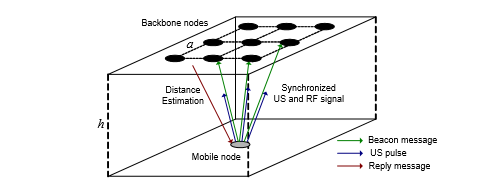
\includegraphics{yonei}
    \caption{Диаграма на разработената система}
    \label{fig:yoneiFig}
\end{figure}

Разработената система в документ \cite{yonei} е класифицирана като активна. За коректно пресмятане на координатите на движещия се компонент се изискват измервания от поне 3 бр. статични компонента. 

В документа е демонстриран метод за корекция на грешки. Тъй като позицията на статичните обекти е константна. При измерване, което е по-голямо от дефинирана константа \textit{MINDISTANCE}, която е равна на височината на помещението. Тъй като обектите се движат по земята разстоянието от средната точка на обекта до сензора е константно (считайки еднакви по форма обекти), ако има засичания които са по-големи от \textit{MINDISTANCE} това означава, че измерването съдържа грешка. За да се коригират данните разстоянието се умножава по константа $\alpha$, която е пропорционална на разликата между измереното разстояние и \textit{MINDISTANCE} [ уравнение \ref{eqMinDist} ]

\begin{equation} \label{eqMinDist}
    d_new = \alpha * \hat{d}
\end{equation}